  % Scripts
% Image scaling: 
% Get-ChildItem figures/*.png,figures/*.jpg,figures/*.jpeg | Foreach { $n = $_.name; ffmpeg -i $_ -vf scale=iw/8:ih/8 figures_lowres/$n }



%\documentclass[journal]{vgtc}                % final (journal style)
%\let\ifpdf\relax
%\documentclass[review,journal]{vgtc}         % review (journal style)
%\documentclass[widereview]{vgtc}             % wide-spaced review
\documentclass[preprint,journal]{vgtc}       % preprint (journal style)

%% Uncomment one of the lines above depending on where your paper is
%% in the conference process. ``review'' and ``widereview'' are for review
%% submission, ``preprint'' is for pre-publication, and the final version
%% doesn't use a specific qualifier.

%% Please use one of the ``review'' options in combination with the
%% assigned online id (see below) ONLY if your paper uses a double blind
%% review process. Some conferences, like IEEE Vis and InfoVis, have NOT
%% in the past.

%% Please note that the use of figures other than the optional teaser is not permitted on the first page
%% of the journal version.  Figures should begin on the second page and be
%% in CMYK or Grey scale format, otherwise, colour shifting may occur
%% during the printing process.  Papers submitted with figures other than the optional teaser on the
%% first page will be refused. Also, the teaser figure should only have the
%% width of the abstract as the template enforces it.

%% These few lines make a distinction between latex and pdflatex calls and they
%% bring in essential packages for graphics and font handling.
%% Note that due to the \DeclareGraphicsExtensions{} call it is no longer necessary
%% to provide the the path and extension of a graphics file:
%% 
\includegraphics{diamondrule} is completely sufficient.
%%
\ifpdf%                                % if we use pdflatex
  \pdfoutput=1\relax                   % create PDFs from pdfLaTeX
  \pdfcompresslevel=9                  % PDF Compression
  \pdfoptionpdfminorversion=7          % create PDF 1.7
  \ExecuteOptions{pdftex}
  \usepackage{graphicx}                % allow us to embed graphics files
  \DeclareGraphicsExtensions{.pdf,.png,.jpg,.jpeg} % for pdflatex we expect .pdf, .png, or .jpg files
\else%                                 % else we use pure latex
  \ExecuteOptions{dvips}
  \usepackage{graphicx}                % allow us to embed graphics files
  \DeclareGraphicsExtensions{.eps}     % for pure latex we expect eps files
\fi%

%% it is recomended to use ``\autoref{sec:bla}'' instead of ``Fig.~\ref{sec:bla}''

\usepackage{microtype}                 % use micro-typography (slightly more compact, better to read)
\PassOptionsToPackage{warn}{textcomp}  % to address font issues with \textrightarrow
\usepackage{textcomp}                  % use better special symbols
\usepackage{mathptmx}                  % use matching math font
\usepackage{times}                     % we use Times as the main font
\renewcommand*\ttdefault{txtt}         % a nicer typewriter font
\usepackage{cite}                      % needed to automatically sort the references
\usepackage{tabu}                      % only used for the table example
\usepackage{booktabs}                  % only used for the table example
%% We encourage the use of mathptmx for consistent usage of times font
%% throughout the proceedings. However, if you encounter conflicts
%% with other math-related packages, you may want to disable it.

\usepackage{amsmath}
\usepackage{amssymb}
\usepackage{xcolor}
%\usepackage{subcaption}
\usepackage{gensymb}

% pic inside the table
%\usepackage{graphicx}% http://ctan.org/pkg/graphicx
\usepackage{array}% http://ctan.org/pkg/array
\usepackage{graphicx}% delete the demo option in your actual code
\usepackage{enumitem}

% Spline
\usepackage{tikz}
\usepackage{pgfplots}
\pgfplotsset{compat=1.12}
\usepgfplotslibrary{fillbetween}

\def\equationautorefname{Eq.}


\newcommand{\joncomment}[1]{\textbf{[JC~} \textcolor{red}{#1} \textbf{~]}}
\newcommand{\alexcomment}[1]{\textbf{[AB~} \textcolor{purple}{#1} \textbf{~]}}
\newcommand{\CS}[1]{\textbf{[CS~} \textcolor{blue}{#1} \textbf{~]}}
\newcommand{\anderscomment}[1]{\textbf{[AY~} \textcolor{cyan}{#1} \textbf{~]}}
\newcommand{\chuckcomment}[1]{\textbf{[CH~} \textcolor{green}{#1} \textbf{~]}}
\newcommand{\etal}{\emph{et al.}}

\newcommand{\alternativeText}[1]{{\textbf{ALTERNATIVE TEXT:}~\color{orange}#1}}

%
% Change this for the final version
%
%\graphicspath{{figures/}{figures_lowres/}{pictures/}}
\graphicspath{{figures_lowres/}{figures/}{pictures/}}

\setlength{\fboxsep}{0pt}


%% In preprint mode you may define your own headline.
%\preprinttext{To appear in IEEE Transactions on Visualization and Computer Graphics.}

%% If you are submitting a paper to a conference for review with a double
%% blind reviewing process, please replace the value ``0'' below with your
%% OnlineID. Otherwise, you may safely leave it at ``0''.
\onlineid{1137}

%% declare the category of your paper, only shown in review mode
\vgtccategory{Research}
%% please declare the paper type of your paper to help reviewers, only shown in review mode
%% choices:
%% * algorithm/technique
%% * application/design study
%% * evaluation
%% * system
%% * theory/model
\vgtcpapertype{algorithm/technique}

%% Paper title.
\title{Supplementary Materials for Interactive Visualization of Atmospheric Effects for Celestial Bodies}

%% This is how authors are specified in the journal style

%% indicate IEEE Member or Student Member in form indicated below
\author{Jonathas Costa, Alexander Bock, Carter Emmart, Charles Hansen, Anders Ynnerman and Cl\'audio Silva, \textit{Member, IEEE}}
\authorfooter{
  \item Jonathas Costa is with New York University. E-mail: jccosta@nyu.edu.  
  \item Alexander Bock is with Link\"oping University and the University of Utah. E-mail: alexander.bock@liu.se.
  \item Carter Emmart is with the American Museum of Natural History. E-mail: carter@amnh.org.
  \item Cl\'audio Silva is with New York University. E-mail: csilva@nyu.edu.
  \item Charles Hansen is with the University of Utah. E-mail: hansen@cs.utah.edu.
  \item Anders Ynnerman is with Link\"oping University and the University of Utah. E-mail: anders.ynnerman@liu.se.
}

\shortauthortitle{Costa \etal: Interactive Visualization of Atmospheric Effects for Celestial Bodies}

%% Keywords that describe your work. Will show as 'Index Terms' in journal
%% please capitalize first letter and insert punctuation after last keyword
\keywords{Physical \& Environmental Sciences, Engineering, Mathematics; Computer Graphics Techniques}

%% ACM Computing Classification System (CCS). 
%% See <http://www.acm.org/class/1998/> for details.
%% The ``\CCScat'' command takes four arguments.

\CCScatlist{ % not used in journal version
 \CCScat{K.6.1}{Management of Computing and Information Systems}%
{Project and People Management}{Life Cycle};
 \CCScat{K.7.m}{The Computing Profession}{Miscellaneous}{Ethics}
}



%% Uncomment below to disable the manuscript note
%\renewcommand{\manuscriptnotetxt}{}

%% Copyright space is enabled by default as required by guidelines.
%% It is disabled by the 'review' option or via the following command:
% \nocopyrightspace

\vgtcinsertpkg

%%%%%%%%%%%%%%%%%%%%%%%%%%%%%%%%%%%%%%%%%%%%%%%%%%%%%%%%%%%%%%%%
%%%%%%%%%%%%%%%%%%%%%% START OF THE PAPER %%%%%%%%%%%%%%%%%%%%%%
%%%%%%%%%%%%%%%%%%%%%%%%%%%%%%%%%%%%%%%%%%%%%%%%%%%%%%%%%%%%%%%%%

\begin{document}

%% The ``\maketitle'' command must be the first command after the
%% ``\begin{document}'' command. It prepares and prints the title block.

\onecolumn
%% the only exception to this rule is the \firstsection command
\firstsection{CIE Curves Validation}
\maketitle


We plot our results for Earth's atmosphere against the CIE clear sky model~\cite{Darula:2002} (model 12, fitted from experimental data). As we can see in \autoref{fig:validation_curves}, our model shows satisfying accuracy and, when compared with models from \cite{BrunetonNeyret:2008, Preetham:1999, Zotti:2007} (whose curves were also available), our model displays the correct (approximate) behavior for higher angles.  Comparisons with varying sun positions and view angles are available in the supplemental material.

\begin{figure*}[!h]
  \centering
  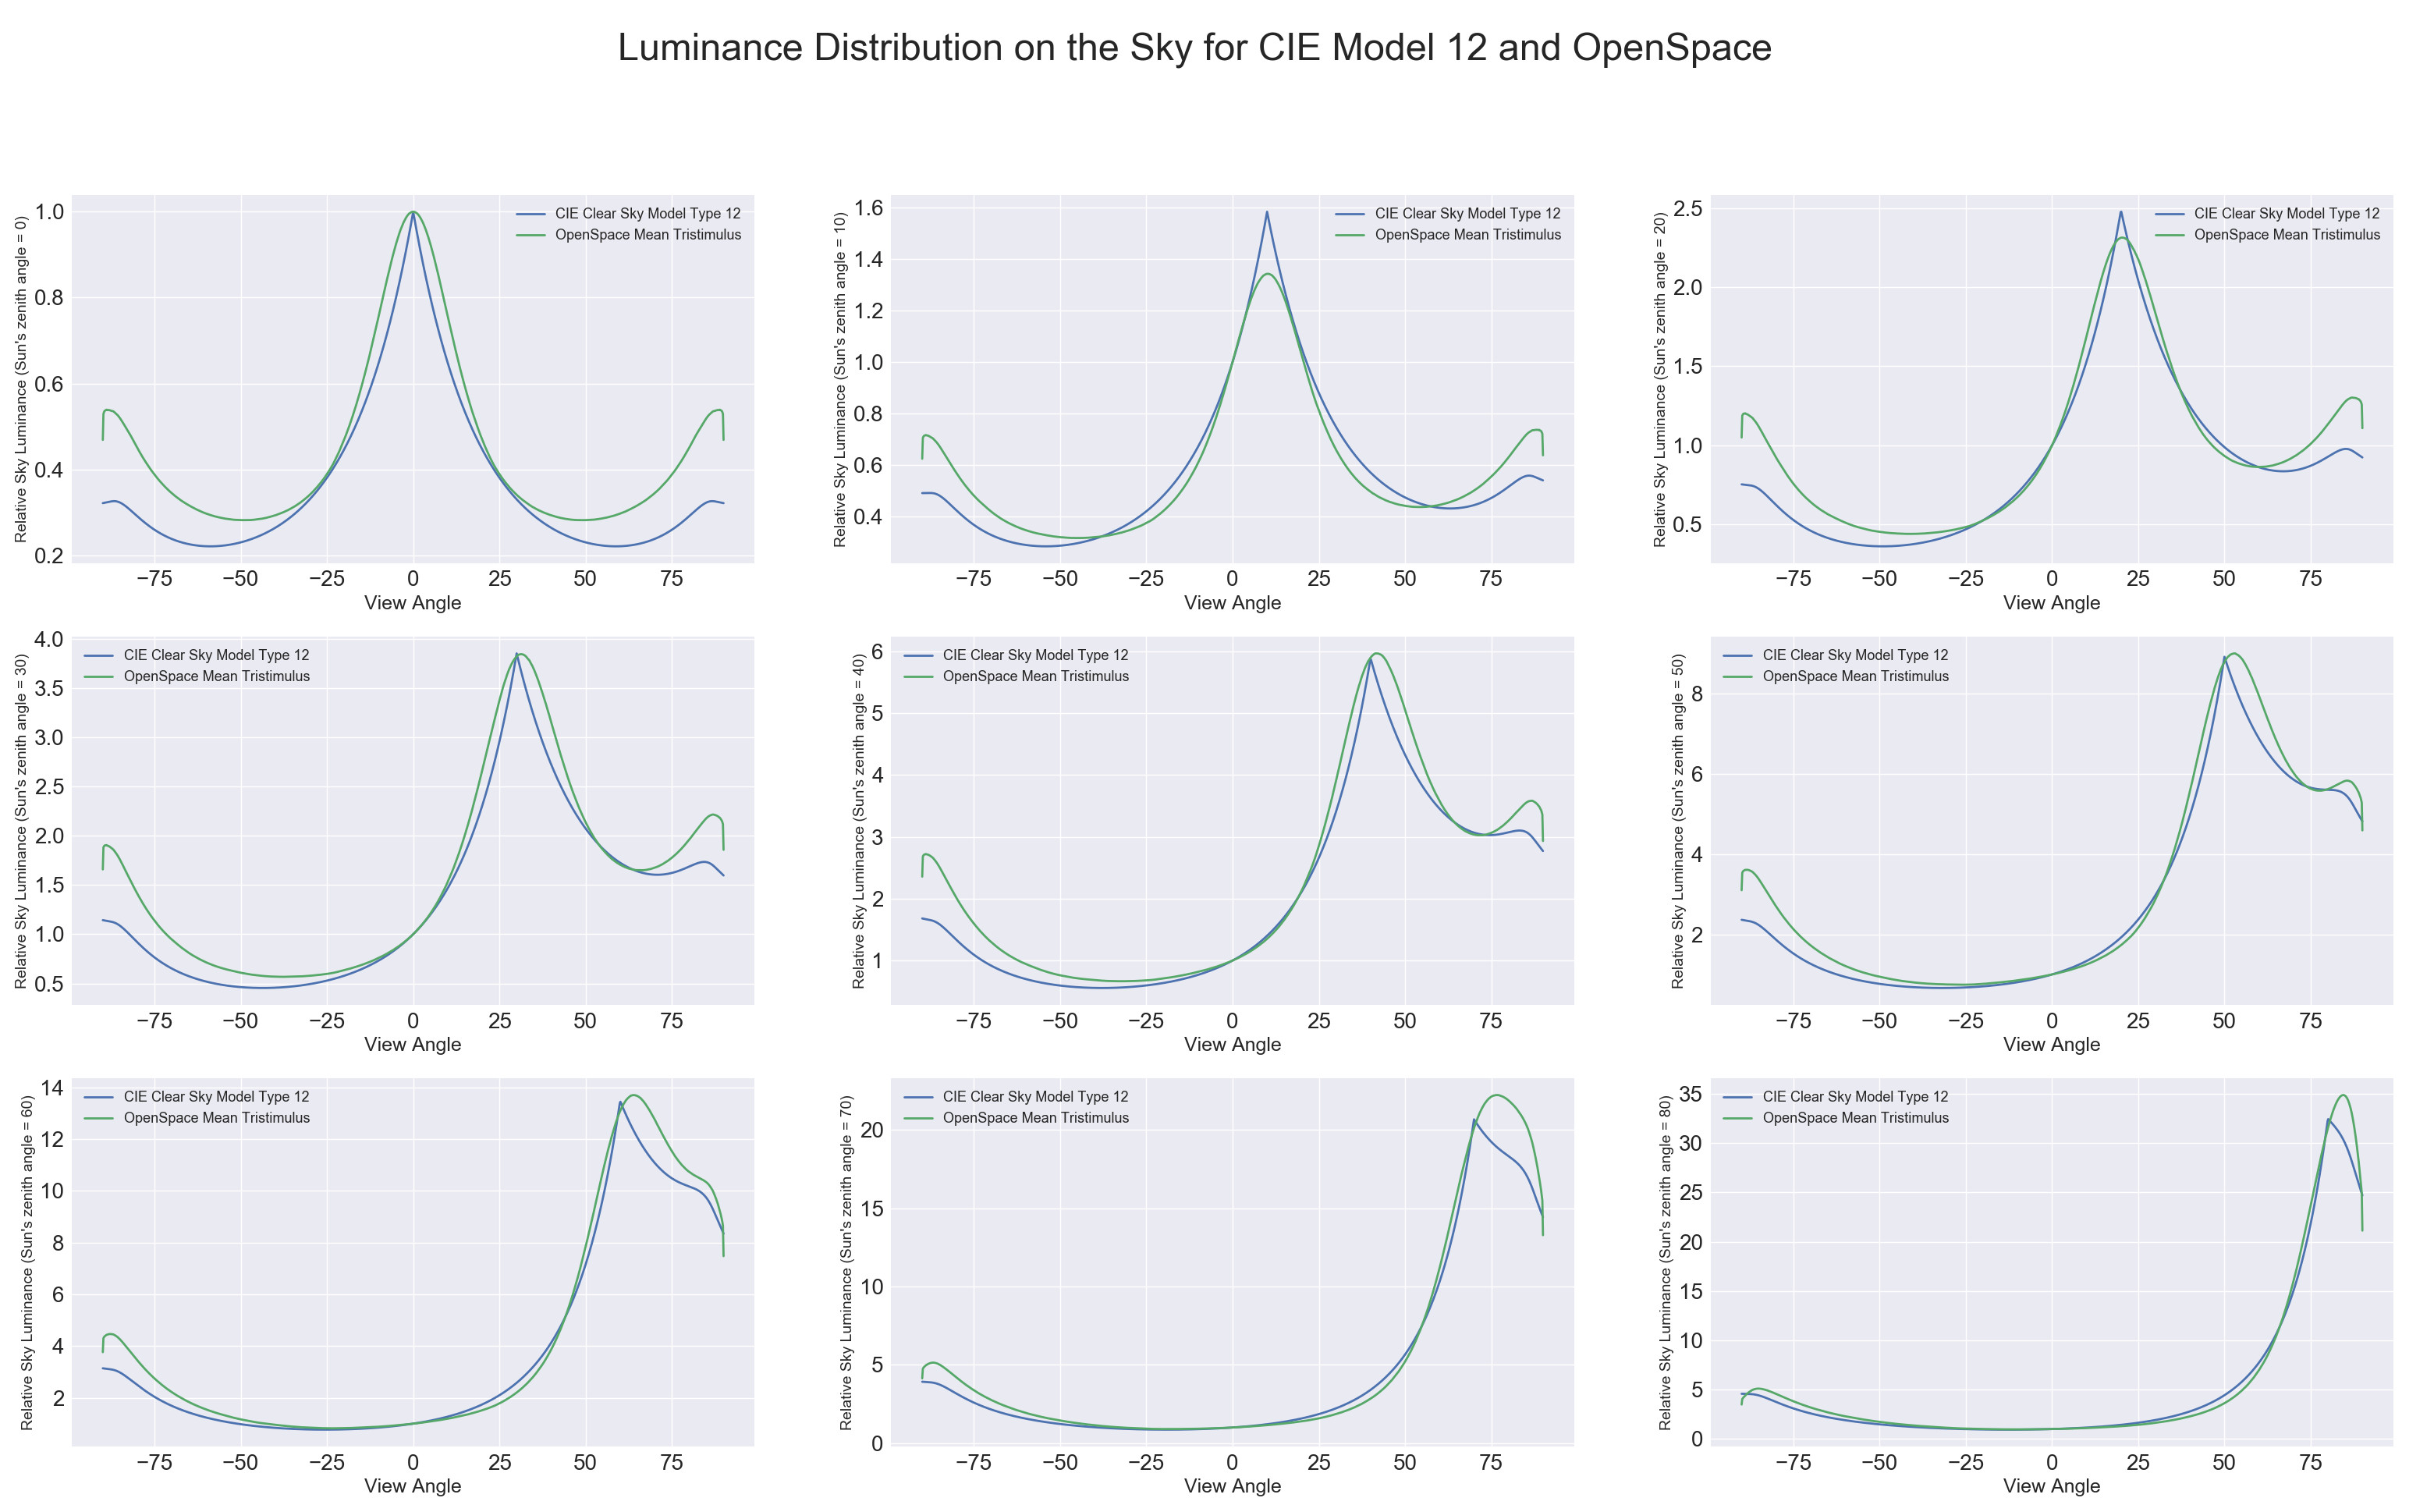
\includegraphics[width=\linewidth]{validation_curves_new.jpg}
  \caption{The sky luminance over the zenith luminance plotted for different sun positions and different view angles into Earth's atmosphere. The blue curve is the CIE Sky modelType 12 (CIE Standard Clear Sky, low luminance turbidity) and the orange line is the results of our advanced parametric model for the atmosphere. Our model agrees well with the CIE's curve and doesn't display the overestimation results near the horizon displayed in other models.}
  \label{fig:validation_curves}
\end{figure*}

\section{Ozone Concentration Cubic Spline}\label{appendix:Ozone}

The ozone layer concentration in molecules per centimeter cubic can be found in~\cite{US_atmosphere:1976}. In order to extract the data for later integration when computing the transmittance values from Eq. 5 in the paper, we fit a piecewise cubic spline over the data. The result is the curve observed in \autoref{fig:ozone-profile} and the function in \autoref{eq:ozone-concentration-spline}.

\begin{figure}
\centering
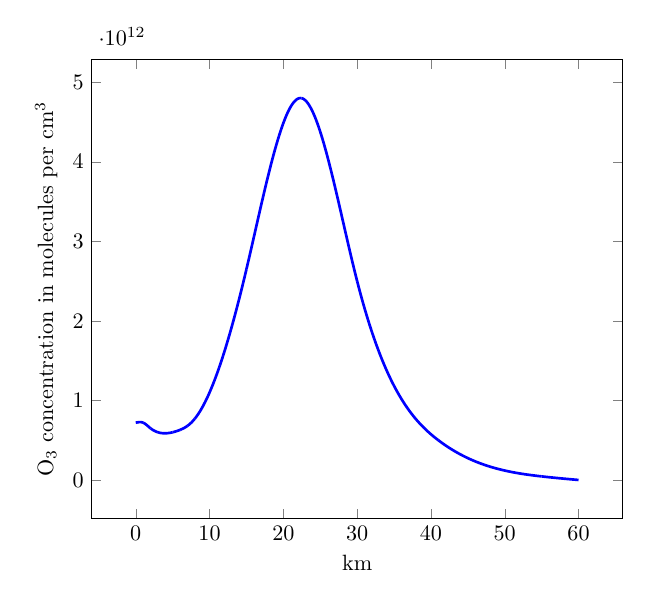
\begin{tikzpicture}[scale=0.8]
	\pgfplotsset{
		scale only axis,
	}

	\begin{axis}[xlabel={km}, ylabel={$\text{O}_3$ concentration in molecules per $\text{cm}^3$}, samples=100,]

%			\addplot [only marks] table {
% data in m^3
%				0 720000000000000000
%				1 720000000000000000
%				2 650000000000000000
%				3 600000000000000000
%				5 600000000000000000
%				6 630000000000000000
%				7 680000000000000000
%				8 770000000000000000
%				15 2650000000000000000
%				22.46 4800000000000000000
%				30 2500000000000000000
%				41 500000000000000000
%				55 45000000000000000
%				60 0
                % data in cm^3
                % 0 720000000000
                % 1 720000000000
                % 2 650000000000
                % 3 600000000000
                % 5 600000000000
                % 6 630000000000
                % 7 680000000000
                % 8 770000000000
                % 15 2650000000000
                % 22.46 4800000000000
                % 30 2500000000000
                % 41 500000000000
                % 55 45000000000
                % 60 0
%			};

    % spline in m^3
% 	\addplot[blue, very thick][domain=0:1]{+-19593973440984870*x^3+-9.199376586608983e-41*x^2+19593973440984870*x^1+720000000000000000*x^0};
% 	\addplot[blue, very thick][domain=1:2]{+27969867204924364*x^3+-142691521937727710*x^2+162285495378712580*x^1+672436159354090800*x^0};
% 	\addplot[blue, very thick][domain=2:3]{+-2285495378712586*x^3+38840653564093990*x^2+-200778855624930800*x^1+914479060023186400*x^0};
% 	\addplot[blue, very thick][domain=3:5]{+-1774770211438684.2*x^3+34244127058628876*x^2+-186989276108535500*x^1+900689480506791000*x^0};
% 	\addplot[blue, very thick][domain=5:6]{+33197493099429.848*x^3+7124611490557163*x^2+-51391698268176910*x^1+674693517439526800*x^0};
% 	\addplot[blue, very thick][domain=6:7]{+4588864760405629*x^3+-74877399320954420*x^2+440620366600892600*x^1+-309330612298612300*x^0};
% 	\addplot[blue, very thick][domain=7:8]{+1611343465278054.2*x^3+-12349452123275350*x^2+2924736217139098*x^1+711959191930145900*x^0};
% 	\addplot[blue, very thick][domain=8:15]{+-620399108377081.1*x^3+41212369644447896*x^2+-425569837924646850*x^1+1854611389641575200*x^0};
% 	\addplot[blue, very thick][domain=15:22.46]{+-3647772872090812*x^3+177444189011565800*x^2+-2469047128431415300*x^1+12071997842175416000*x^0};
% 	\addplot[blue, very thick][domain=22.46:30]{+4026153507212336.5*x^3+-339624970425880300*x^2+9144326192533625000*x^1+-74873457087449510000*x^0};
% 	\addplot[blue, very thick][domain=30:41]{+-572544758081184.8*x^3+74257873450536560*x^2+-3272159123758882300*x^1+49291396075475560000*x^0};
% 	\addplot[blue, very thick][domain=41:55]{+-80772648333736.36*x^3+13769903951600404*x^2+-792152374302500000*x^1+15397970499571663000*x^0};
% 	\addplot[blue, very thick][domain=55:60]{+-29494465102260.28*x^3+5309003718406851*x^2+-326802861476854500*x^1+6866562764434830000*x^0};		
	% spline in cm^3
    \addplot[blue, very thick][domain=0:1]{+-19593973440.984875*x^3+-9.199376586608983e-47*x^2+19593973440.984875*x^1+720000000000*x^0};
	\addplot[blue, very thick][domain=1:2]{+27969867204.924366*x^3+-142691521937.72772*x^2+162285495378.7126*x^1+672436159354.0908*x^0};
	\addplot[blue, very thick][domain=2:3]{+-2285495378.712586*x^3+38840653564.093994*x^2+-200778855624.93082*x^1+914479060023.1864*x^0};
	\addplot[blue, very thick][domain=3:5]{+-1774770211.4386845*x^3+34244127058.628876*x^2+-186989276108.5355*x^1+900689480506.791*x^0};
	\addplot[blue, very thick][domain=5:6]{+33197493.099429846*x^3+7124611490.557163*x^2+-51391698268.17691*x^1+674693517439.5267*x^0};
	\addplot[blue, very thick][domain=6:7]{+4588864760.405629*x^3+-74877399320.95442*x^2+440620366600.8926*x^1+-309330612298.61224*x^0};
	\addplot[blue, very thick][domain=7:8]{+1611343465.2780542*x^3+-12349452123.27535*x^2+2924736217.139098*x^1+711959191930.1459*x^0};
	\addplot[blue, very thick][domain=8:15]{+-620399108.3770812*x^3+41212369644.4479*x^2+-425569837924.64685*x^1+1854611389641.5752*x^0};
	\addplot[blue, very thick][domain=15:22.46]{+-3647772872.0908117*x^3+177444189011.56577*x^2+-2469047128431.415*x^1+12071997842175.416*x^0};
	\addplot[blue, very thick][domain=22.46:30]{+4026153507.2123365*x^3+-339624970425.8804*x^2+9144326192533.625*x^1+-74873457087449.52*x^0};
	\addplot[blue, very thick][domain=30:41]{+-572544758.0811847*x^3+74257873450.53656*x^2+-3272159123758.8823*x^1+49291396075475.555*x^0};
	\addplot[blue, very thick][domain=41:55]{+-80772648.33373636*x^3+13769903951.600403*x^2+-792152374302.5*x^1+15397970499571.662*x^0};
	\addplot[blue, very thick][domain=55:60]{+-29494465.10226028*x^3+5309003718.406851*x^2+-326802861476.85455*x^1+6866562764434.83*x^0};
		
	\end{axis}
\end{tikzpicture}
\caption{The Ozone layer profile concentration in function of height (in $km$). Curve generated fitting a piecewise cubic spline over the data from~\cite{US_atmosphere:1976}.} \label{fig:ozone-profile}
\end{figure}

\begin{equation}
    \rho_{O_3}(h) = \begin{cases}-1.9594 \cdot 10^{10}\cdot x^3 + -9.1994 \cdot 10^{-47}\cdot x^2 + 1.9594 \cdot 10^{10}\cdot x + 7.2000 \cdot 10^{11}, & \text{if } x \in [0,1], \\2.7970 \cdot 10^{10}\cdot x^3 + -1.4269 \cdot 10^{11}\cdot x^2 + 1.6229 \cdot 10^{11}\cdot x + 6.7244 \cdot 10^{11}, & \text{if } x \in (1,2], \\-2.2855 \cdot 10^{9}\cdot x^3 + 3.8841 \cdot 10^{10}\cdot x^2 + -2.0078 \cdot 10^{11}\cdot x + 9.1448 \cdot 10^{11}, & \text{if } x \in (2,3], \\-1.7748 \cdot 10^{9}\cdot x^3 + 3.4244 \cdot 10^{10}\cdot x^2 + -1.8699 \cdot 10^{11}\cdot x + 9.0069 \cdot 10^{11}, & \text{if } x \in (3,5], \\3.3197 \cdot 10^{7}\cdot x^3 + 7.1246 \cdot 10^{9}\cdot x^2 + -5.1392 \cdot 10^{10}\cdot x + 6.7469 \cdot 10^{11}, & \text{if } x \in (5,6], \\4.5889 \cdot 10^{9}\cdot x^3 + -7.4877 \cdot 10^{10}\cdot x^2 + 4.4062 \cdot 10^{11}\cdot x + -3.0933 \cdot 10^{11}, & \text{if } x \in (6,7], \\1.6113 \cdot 10^{9}\cdot x^3 + -1.2349 \cdot 10^{10}\cdot x^2 + 2.9247 \cdot 10^{9}\cdot x + 7.1196 \cdot 10^{11}, & \text{if } x \in (7,8], \\-6.2040 \cdot 10^{8}\cdot x^3 + 4.1212 \cdot 10^{10}\cdot x^2 + -4.2557 \cdot 10^{11}\cdot x + 1.8546 \cdot 10^{12}, & \text{if } x \in (8,15], \\-3.6478 \cdot 10^{9}\cdot x^3 + 1.7744 \cdot 10^{11}\cdot x^2 + -2.4690 \cdot 10^{12}\cdot x + 1.2072 \cdot 10^{13}, & \text{if } x \in (15,22.46], \\4.0262 \cdot 10^{9}\cdot x^3 + -3.3962 \cdot 10^{11}\cdot x^2 + 9.1443 \cdot 10^{12}\cdot x + -7.4873 \cdot 10^{13}, & \text{if } x \in (22.46,30], \\-5.7254 \cdot 10^{8}\cdot x^3 + 7.4258 \cdot 10^{10}\cdot x^2 + -3.2722 \cdot 10^{12}\cdot x + 4.9291 \cdot 10^{13}, & \text{if } x \in (30,41], \\-8.0773 \cdot 10^{7}\cdot x^3 + 1.3770 \cdot 10^{10}\cdot x^2 + -7.9215 \cdot 10^{11}\cdot x + 1.5398 \cdot 10^{13}, & \text{if } x \in (41,55], \\-2.9494 \cdot 10^{7}\cdot x^3 + 5.3090 \cdot 10^{9}\cdot x^2 + -3.2680 \cdot 10^{11}\cdot x + 6.8666 \cdot 10^{12}, & \text{if } x \in (55,60].\end{cases}
    \label{eq:ozone-concentration-spline}
\end{equation}

% Curve in m^3
    % f(x) = \begin{cases}-1.9594 \cdot 10^{16}\cdot x^3 + -9.1994 \cdot 10^{-41}\cdot x^2 + 1.9594 \cdot 10^{16}\cdot x + 7.2000 \cdot 10^{17}, & \text{if } x \in [0,1], \\2.7970 \cdot 10^{16}\cdot x^3 + -1.4269 \cdot 10^{17}\cdot x^2 + 1.6229 \cdot 10^{17}\cdot x + 6.7244 \cdot 10^{17}, & \text{if } x \in (1,2], \\-2.2855 \cdot 10^{15}\cdot x^3 + 3.8841 \cdot 10^{16}\cdot x^2 + -2.0078 \cdot 10^{17}\cdot x + 9.1448 \cdot 10^{17}, & \text{if } x \in (2,3], \\-1.7748 \cdot 10^{15}\cdot x^3 + 3.4244 \cdot 10^{16}\cdot x^2 + -1.8699 \cdot 10^{17}\cdot x + 9.0069 \cdot 10^{17}, & \text{if } x \in (3,5], \\3.3197 \cdot 10^{13}\cdot x^3 + 7.1246 \cdot 10^{15}\cdot x^2 + -5.1392 \cdot 10^{16}\cdot x + 6.7469 \cdot 10^{17}, & \text{if } x \in (5,6], \\4.5889 \cdot 10^{15}\cdot x^3 + -7.4877 \cdot 10^{16}\cdot x^2 + 4.4062 \cdot 10^{17}\cdot x + -3.0933 \cdot 10^{17}, & \text{if } x \in (6,7], \\1.6113 \cdot 10^{15}\cdot x^3 + -1.2349 \cdot 10^{16}\cdot x^2 + 2.9247 \cdot 10^{15}\cdot x + 7.1196 \cdot 10^{17}, & \text{if } x \in (7,8], \\-6.2040 \cdot 10^{14}\cdot x^3 + 4.1212 \cdot 10^{16}\cdot x^2 + -4.2557 \cdot 10^{17}\cdot x + 1.8546 \cdot 10^{18}, & \text{if } x \in (8,15], \\-3.6478 \cdot 10^{15}\cdot x^3 + 1.7744 \cdot 10^{17}\cdot x^2 + -2.4690 \cdot 10^{18}\cdot x + 1.2072 \cdot 10^{19}, & \text{if } x \in (15,22.46], \\4.0262 \cdot 10^{15}\cdot x^3 + -3.3962 \cdot 10^{17}\cdot x^2 + 9.1443 \cdot 10^{18}\cdot x + -7.4873 \cdot 10^{19}, & \text{if } x \in (22.46,30], \\-5.7254 \cdot 10^{14}\cdot x^3 + 7.4258 \cdot 10^{16}\cdot x^2 + -3.2722 \cdot 10^{18}\cdot x + 4.9291 \cdot 10^{19}, & \text{if } x \in (30,41], \\-8.0773 \cdot 10^{13}\cdot x^3 + 1.3770 \cdot 10^{16}\cdot x^2 + -7.9215 \cdot 10^{17}\cdot x + 1.5398 \cdot 10^{19}, & \text{if } x \in (41,55], \\-2.9494 \cdot 10^{13}\cdot x^3 + 5.3090 \cdot 10^{15}\cdot x^2 + -3.2680 \cdot 10^{17}\cdot x + 6.8666 \cdot 10^{18}, & \text{if } x \in (55,60].\end{cases}


\section{Performance}

In order to analyze the performance scalability of our method, we plotted the rendering performance (in average frames per second) against the number of simultaneously visible atmospheres in \autoref{fig:scalability_plot}.

\begin{figure}[tbh]
  \centering
  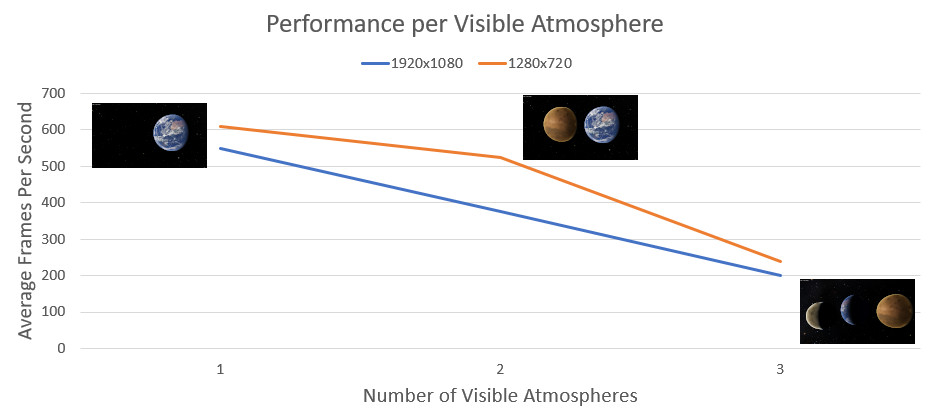
\includegraphics[width=0.6\linewidth]{scalability.jpg}
  \caption{Plotting the performance of our implementation relative to the number of visible atmospheres. The Y-axis is the average frame rate per second for one, two, or three visible atmospheres rendered simultaneously.}
  \label{fig:scalability_plot}
\end{figure}

For the second set of data (\autoref{tbl:data}), we extract the performance (in average frames per second for a 10s period) of our method in OpenSpace for different simultaneous atmospheres.

\begin{table}[h!]
	\begin{center}
     	\begin{tabular}{ p{4.5cm} p{4cm} p{2.5cm} p{2.5cm} }
		\toprule
      	Screenshot & Scene & Res 1280x720 & Res 1920x1080 \\ 
	    \cmidrule(r){1-1}\cmidrule(lr){2-2}\cmidrule(l){3-3}\cmidrule(l){4-4}
    	 \raisebox{-\totalheight}{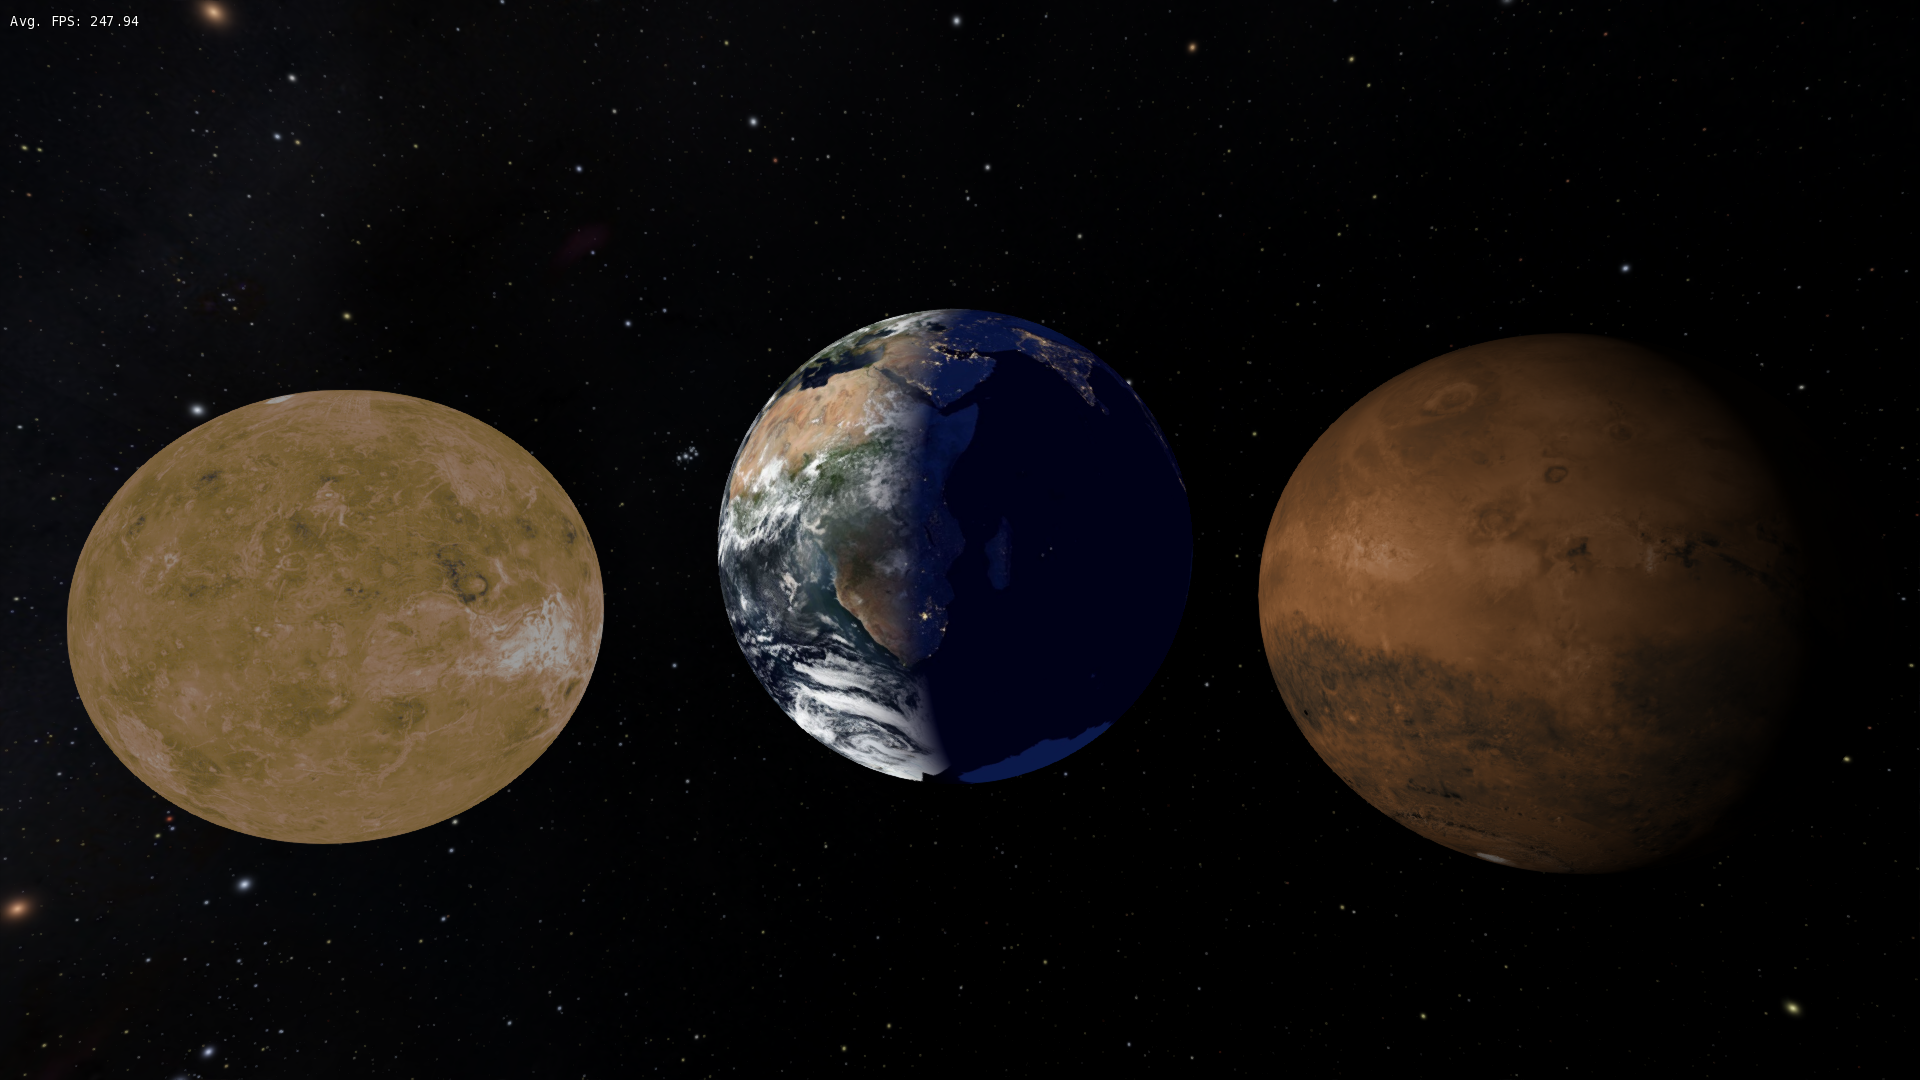
\includegraphics[width=0.25\textwidth, height=29mm]{OpenSpace_3-planets-new.png}}
      	&
      	Three planets, no atmospheres
      	&
	    4.16\,ms (240 FPS)
      	& 
      	3.57\,ms (280 FPS)\\     	
	    \cmidrule(r){1-1}\cmidrule(lr){2-2}\cmidrule(l){3-3}\cmidrule(l){4-4}
    	 \raisebox{-\totalheight}{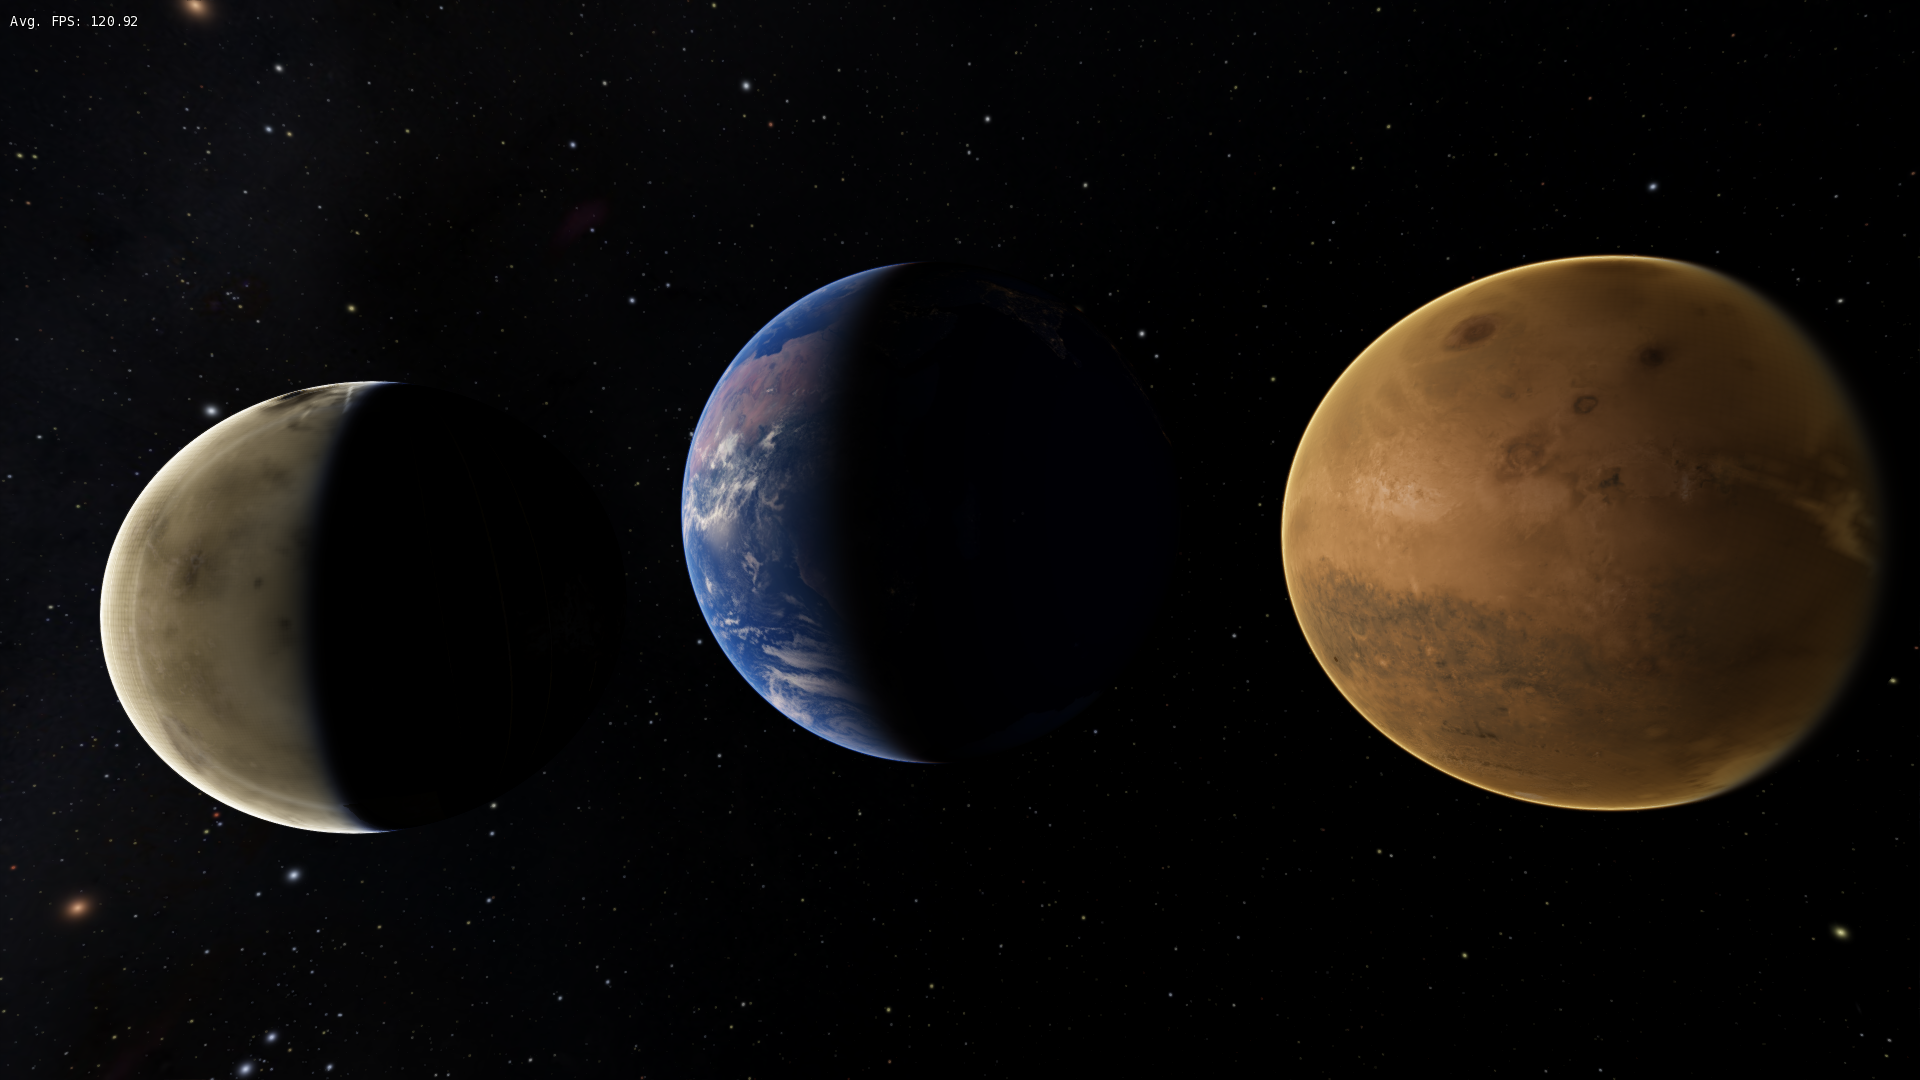
\includegraphics[width=0.25\textwidth, height=29mm]{OpenSpace_000010.png}}
      	& 
      	Three planets, three atmospheres
      	&
	    5\,ms (200 FPS)
      	& 
      	6.06\,ms (165 FPS)\\     	
	    \cmidrule(r){1-1}\cmidrule(lr){2-2}\cmidrule(l){3-3}\cmidrule(l){4-4}
    	 \raisebox{-\totalheight}{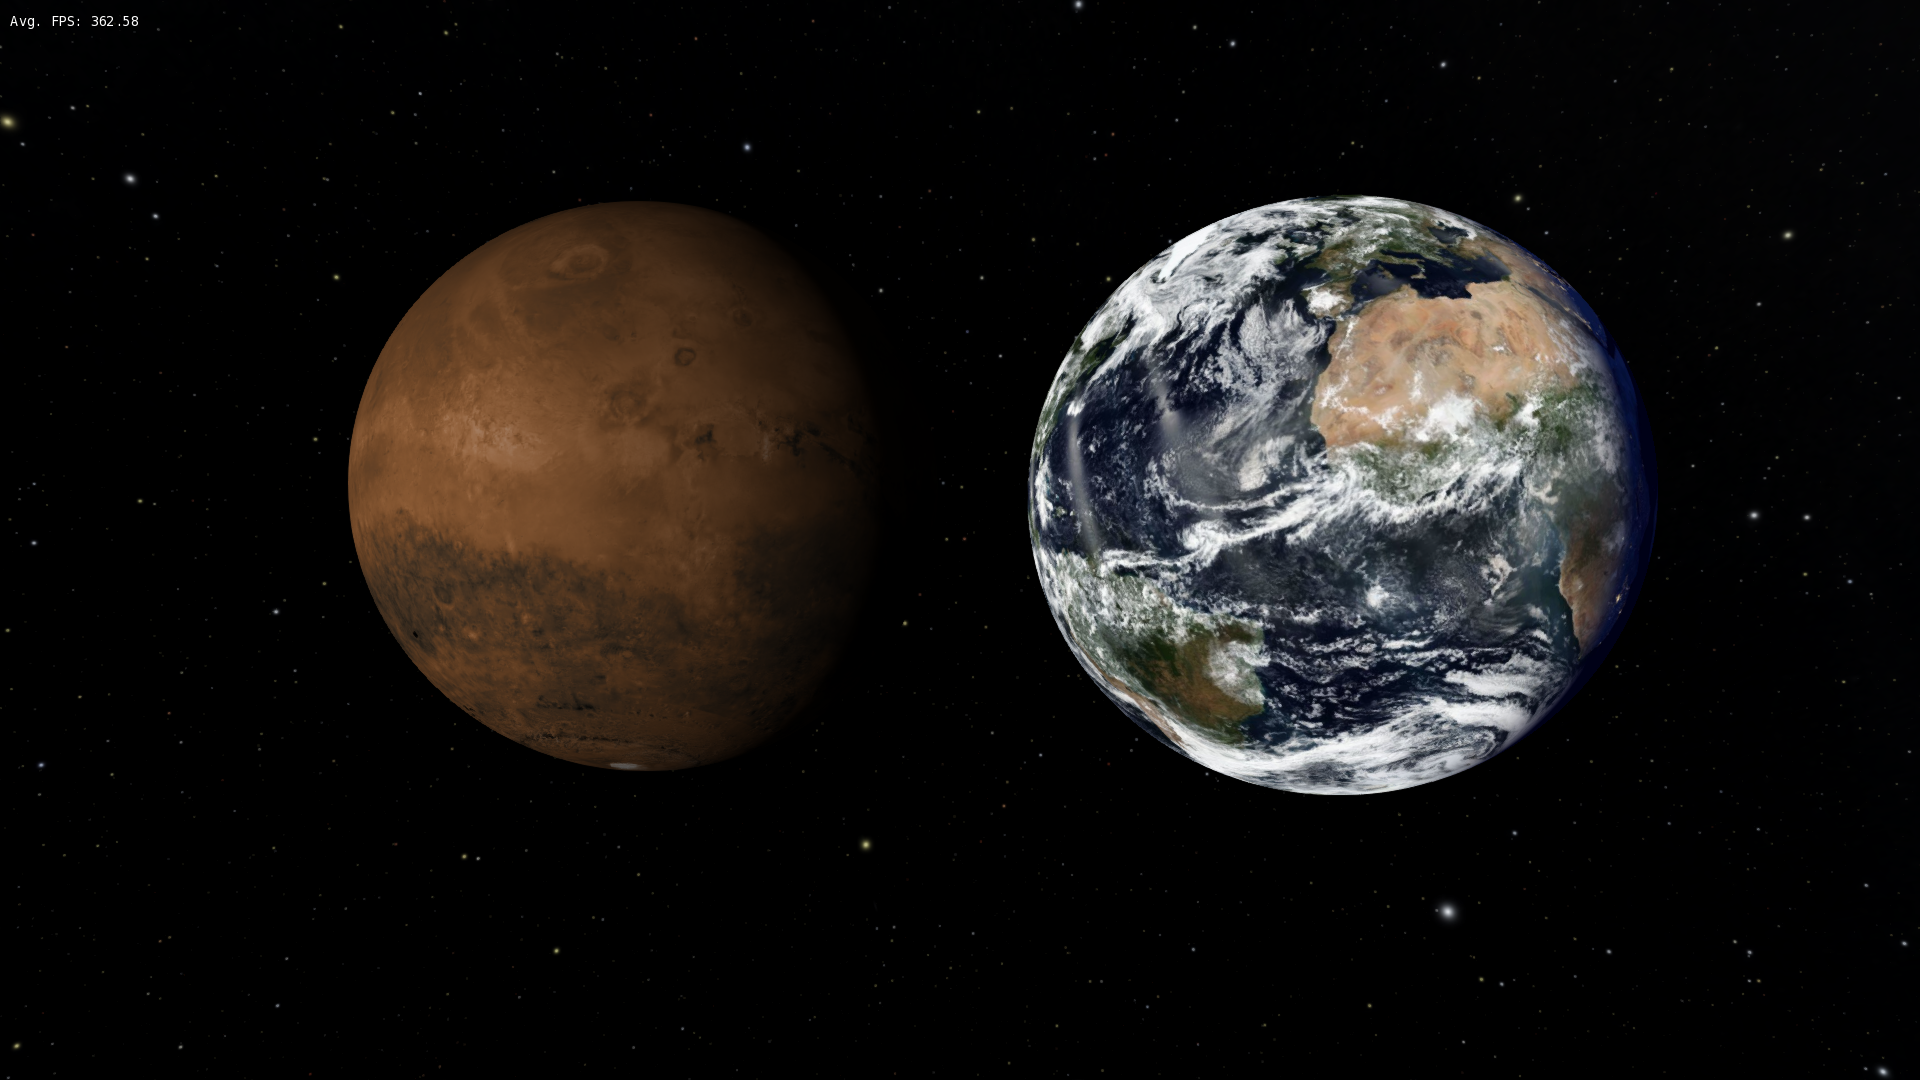
\includegraphics[width=0.25\textwidth, height=29mm]{OpenSpace_000008.png}}
      	& 
      	Two planets, no atmospheres
      	&
	    1.91\,ms (523 FPS)
      	& 
      	2.56\,ms (390 FPS)\\
      	\cmidrule(r){1-1}\cmidrule(lr){2-2}\cmidrule(l){3-3}\cmidrule(l){4-4}
    	 \raisebox{-\totalheight}{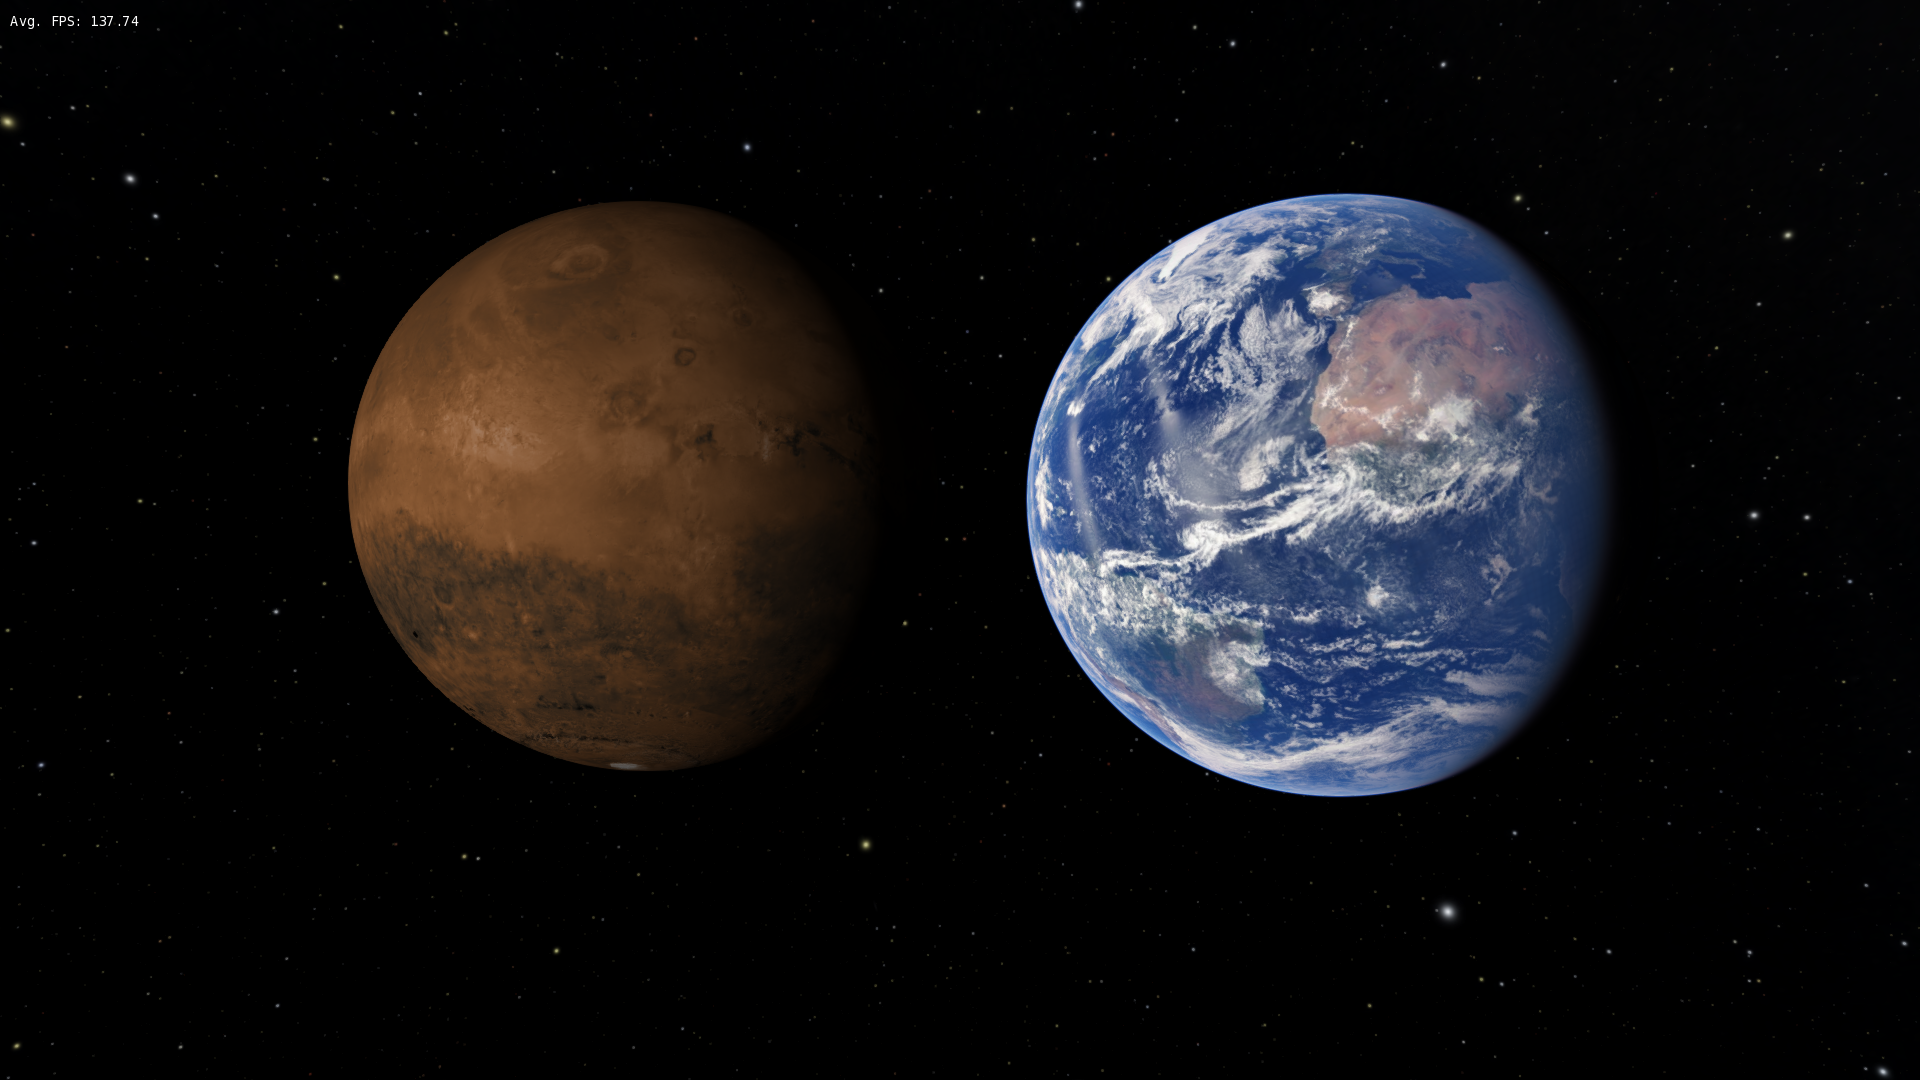
\includegraphics[width=0.25\textwidth, height=29mm]{OpenSpace_000007.png}}
      	& 
      	Two planets, one atmosphere
      	&
	    2.38\,ms (420 FPS)
      	& 
      	3.57\,ms (280 FPS)\\
      	\cmidrule(r){1-1}\cmidrule(lr){2-2}\cmidrule(l){3-3}\cmidrule(l){4-4}
    	 \raisebox{-\totalheight}{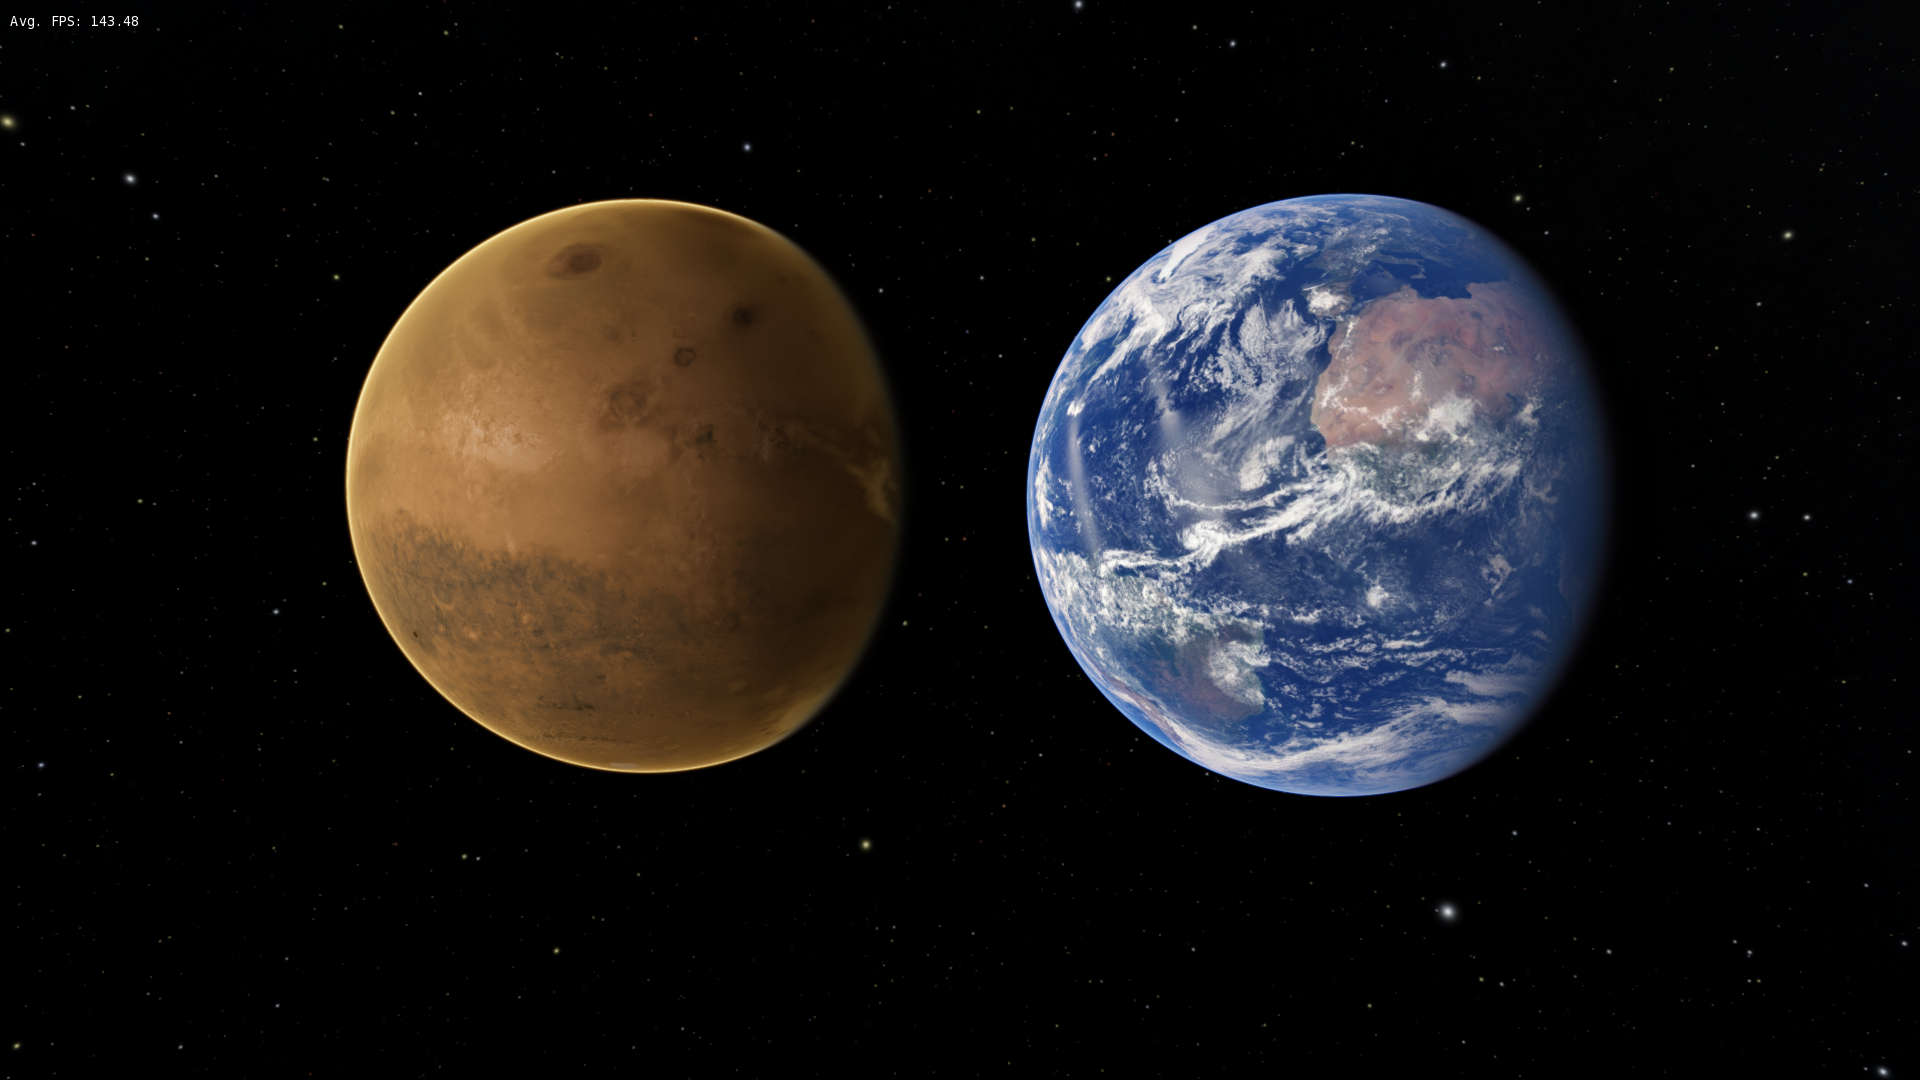
\includegraphics[width=0.25\textwidth, height=29mm]{OpenSpace_000006.png}}
      	& 
      	Two planets, two atmospheres
      	&
	    2.66\,ms (376 FPS)
      	& 
      	4.08\,ms (245 FPS)\\
      	\cmidrule(r){1-1}\cmidrule(lr){2-2}\cmidrule(l){3-3}\cmidrule(l){4-4}
    	 \raisebox{-\totalheight}{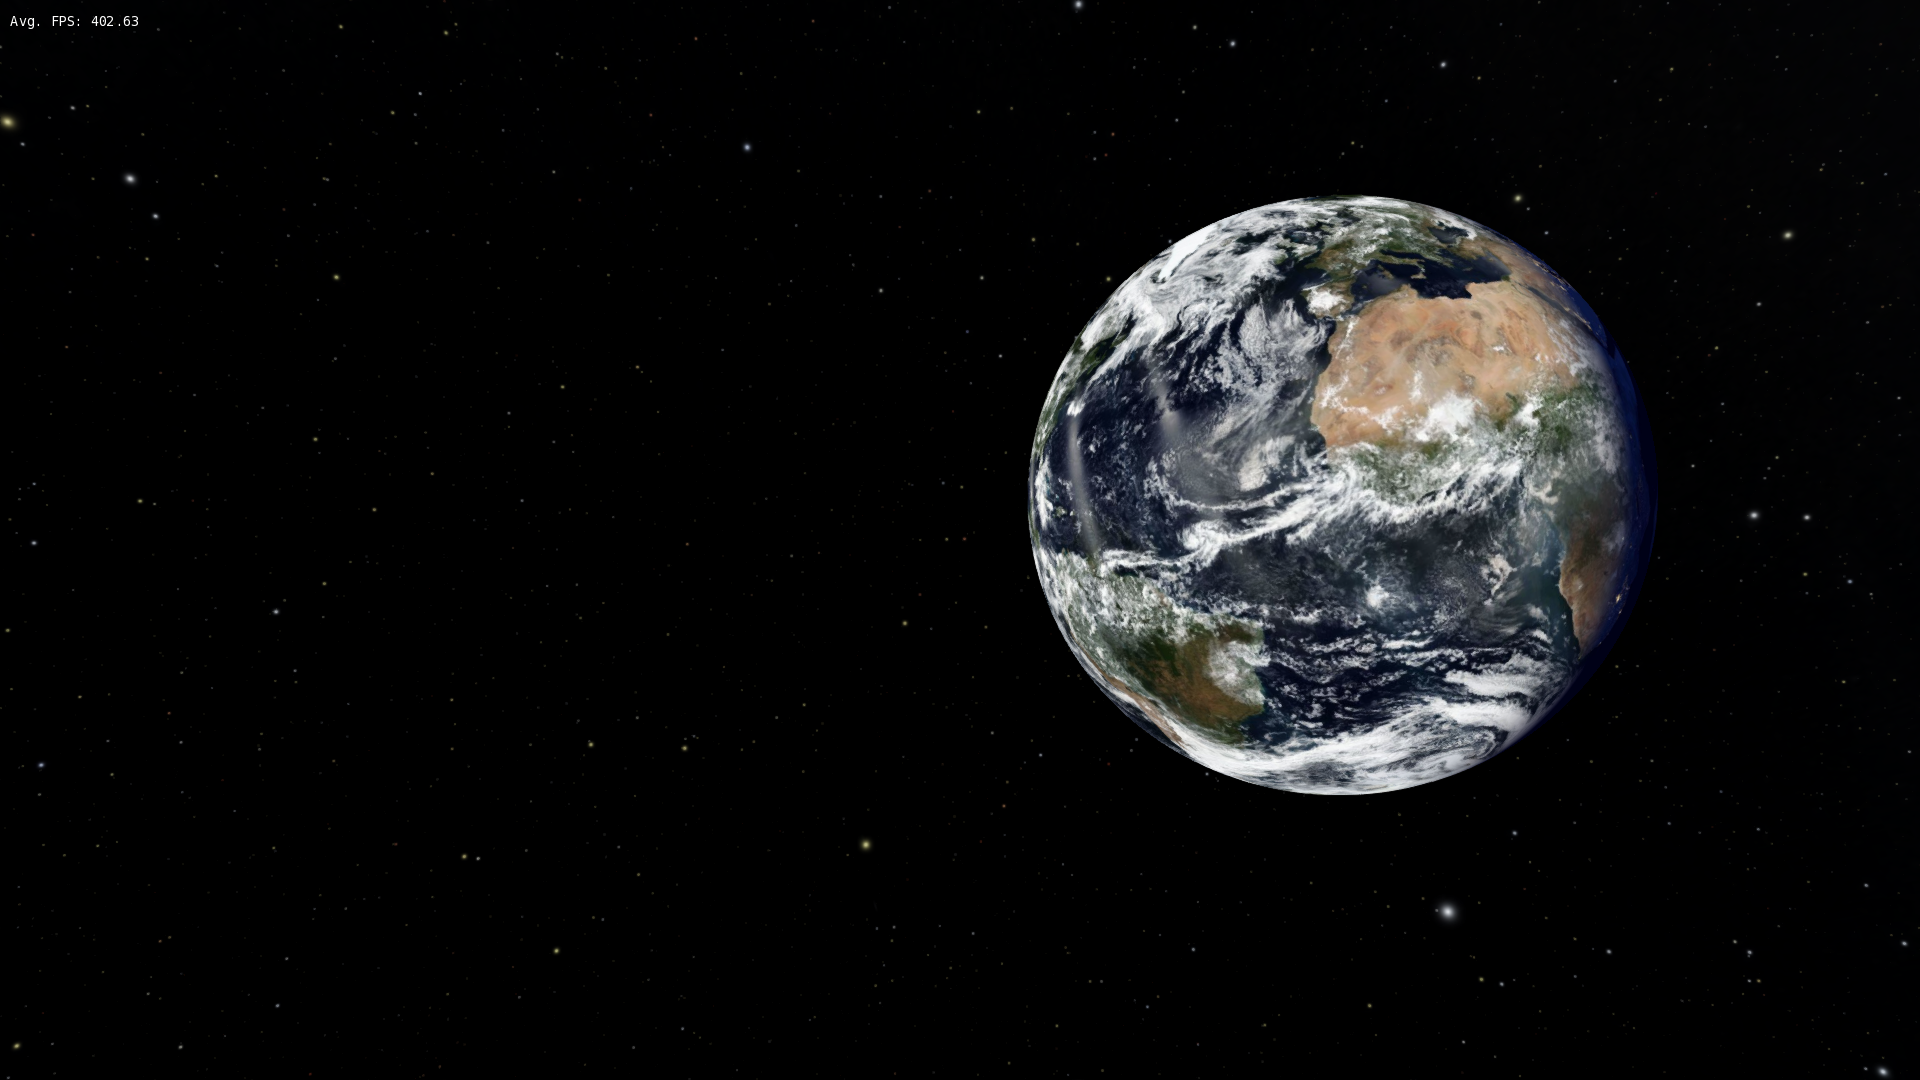
\includegraphics[width=0.25\textwidth, height=29mm]{OpenSpace_000005.png}}
      	& 
      	One planet, no atmosphere
      	&
	    1.64\,ms (610 FPS)
      	& 
      	1.81\,ms (550 FPS)\\
      	\cmidrule(r){1-1}\cmidrule(lr){2-2}\cmidrule(l){3-3}\cmidrule(l){4-4}
    	 \raisebox{-\totalheight}{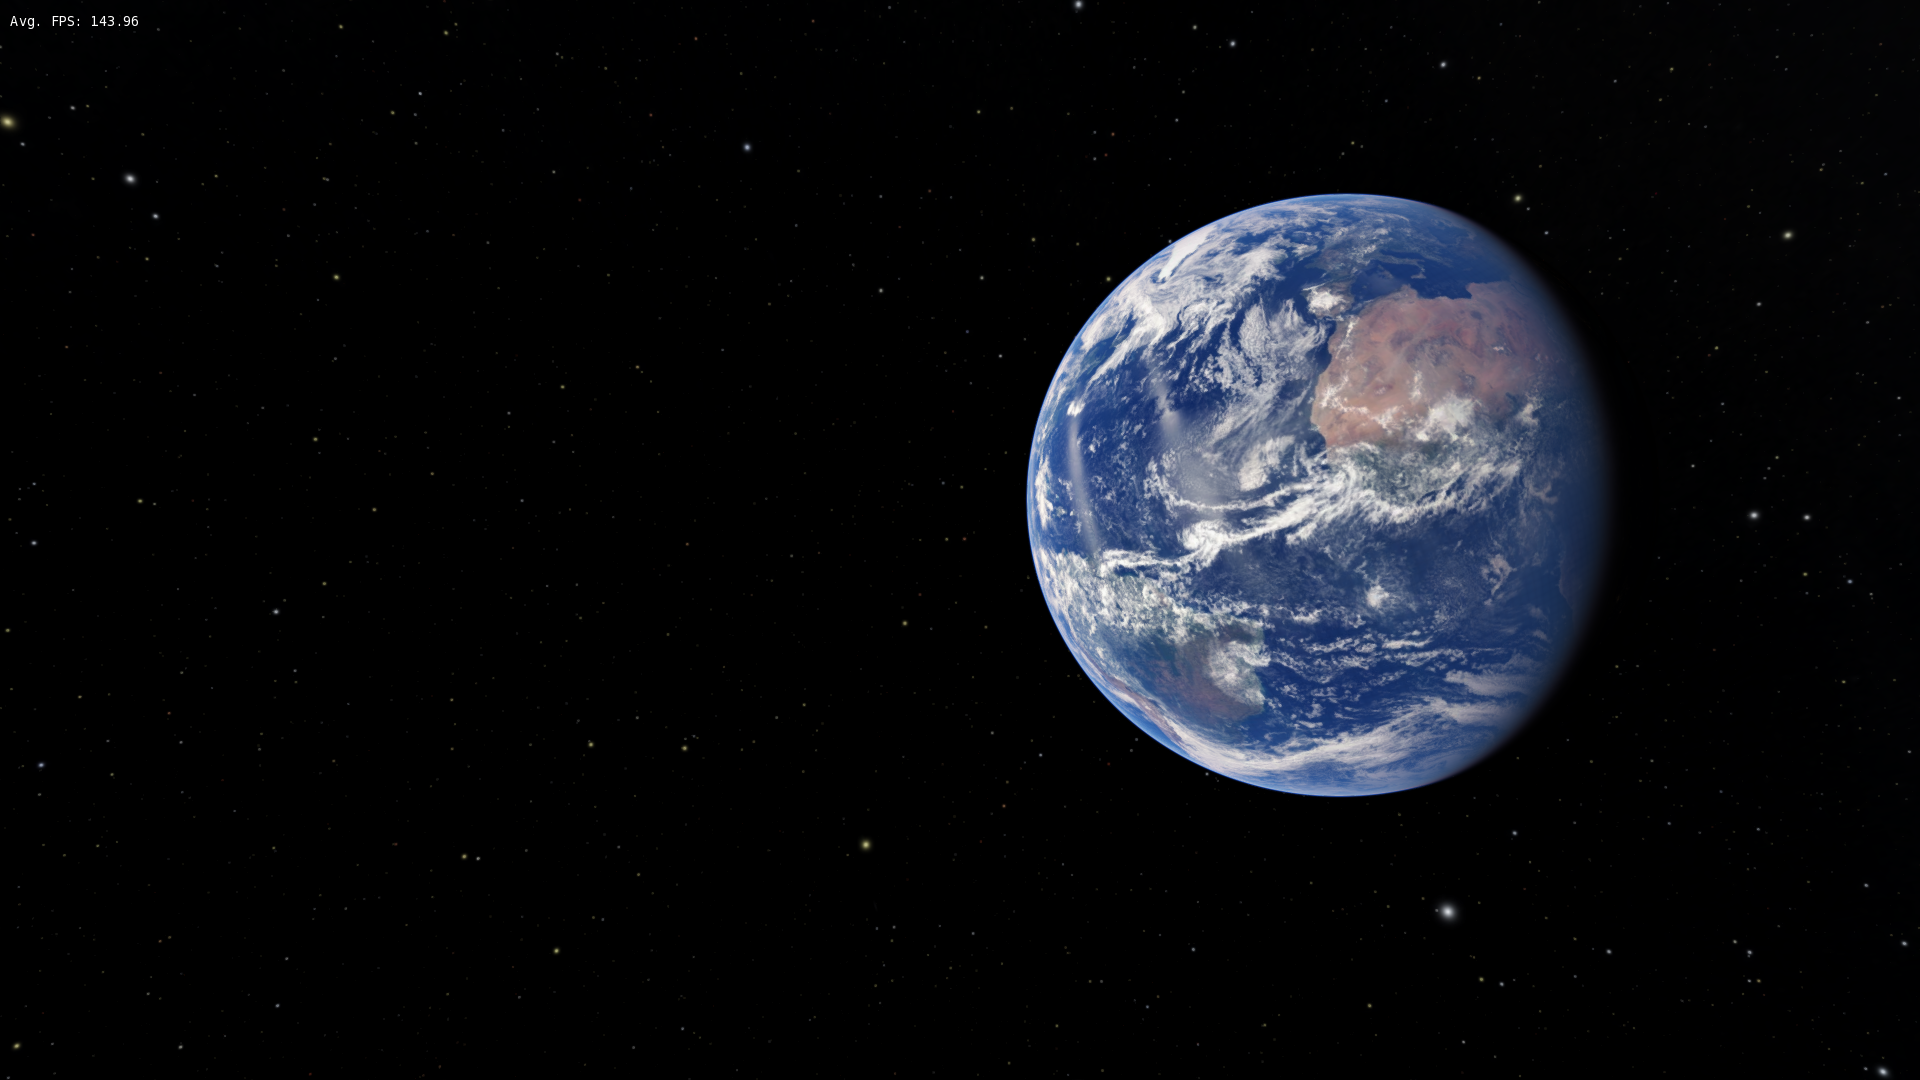
\includegraphics[width=0.25\textwidth, height=29mm]{OpenSpace_000004.png}}
      	& 
      	One planet, one atmosphere
      	&
	    1.81\,ms (550 FPS)
      	& 
      	2.63\,ms (380 FPS)
      	\\ \bottomrule
      \end{tabular}
      \caption{Performance data extracted from the OpenSpace system running the implementation of our model. The performance values describe the mean of the average frame rate per second for 10 seconds for two different resolutions.}
      \label{tbl:data}
   \end{center}
\end{table}

%%%%%%%%%%%%%%%%%%%%%%%%%%%%%%%%%%%%%%%%%%%%%%%%%%%%%%%%%%%%%%%%%%%%%%
%% if specified like this the section will be committed in review mode
%\acknowledgments{
%The authors wish to thank A, B, and C. This work was supported in part by
%a grant from XYZ (\# 12345-67890).}

%%%%%%%%%%%%%%%%%%%%%%%%%%%%%%%%%%%%%%%%%%%%%%%%%%%%%%%%%%%%%%%%%%%%%
%\bibliographystyle{abbrv}
\bibliographystyle{abbrv-doi}
%\bibliographystyle{abbrv-doi-narrow}
%\bibliographystyle{abbrv-doi-hyperref}
%\bibliographystyle{abbrv-doi-hyperref-narrow}

\bibliography{main}
\end{document}

